\documentclass[a4paper,12pt]{article}

%% PACKAGES %%
\usepackage{usenix,graphicx,times,fancyhdr,algorithm,algorithmic,url}
\usepackage[left=1in,top=1in,right=1in,bottom=1in]{geometry}
\graphicspath{{./images/}}

%% MY COMMANDS %%
\newcommand{\projecttitle}{Erg OCR}
\newcommand{\projectsubtitle}{A Machine Learning Approach to Recording Workouts}

%% DOCUMENT START %%
\begin{document}

% page numbers and headers
\thispagestyle{plain}
\pagestyle{fancy}
\clearpage
\setlength{\headsep}{0.4in}


\title{Erg OCR\\ \large A Machine Learning Apprach to Recording Workouts}
\date{\today}
\author{
  {\rm Erik Kessler}\\
  Williams College\\
  Fall 2016
}

\maketitle

\lhead{CS 373}
\chead{\projecttitle}
\rhead{Kessler}
\cfoot{\thepage}

\begin{abstract}
We created a program to convert pictures of Concept2 erg screens into a computer readable format for workout logging and performance tracking. Our system takes a image of an erg screen and is able to determine the location of characters on the screen. The system then does optical character recognition using a k-nearest neighbors machine learning algorithm to determine what characters are at those locations. When the picture is well framed and correctly rotated, our system successfully reads workout data from the picture.
\end{abstract}


\section{Introduction}
Concept2 Ergometers (ergs) are a popular training tool for rowing teams across the world. Furthermore, the data that working out on these machines produces is often used to quantify the strength of a rower. As a result, tracking improvement on this machine is important for rowers and rowing teams. After completing a workout, athletes will often navigate, on the machine\rq s built-in monitor, to a screen that shows a summary of their workout. The athlete must then manually input the data from the screen into their smartphone for tracking. This manual process is time consuming as the erg records many metrics. Therefore, many athletes simply do not record their progress because it is too time consuming and takes athletes out of the flow of the workout.

\begin{figure}[h]
    \centering
    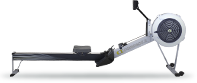
\includegraphics[width=.35\textwidth]{erg}
    \includegraphics[width=.2\textwidth]{pm5_3}
    \caption{An erg and an example of a workout summary screen.}
    \label{fig:erg}
\end{figure}

There is value in having the ability to quickly and seamlessly track workouts with minimal setup or disruption. The goal of this project was to develop a system that could extract workout data from the picture of an Concept2 erg workout summary screen using optical character recognition (OCR) with the goal of allowing users to easily get their workout data onto their phone where other applications can then use it for logging, progress tracking, and team competitions.


\section{Related Work}
First, we discuss why OCR is the technology we want to work with. Concept2 has recently added  bluetooth to their monitors, so bluetooth would be a possible way to get data to the phone. However, we have previously explored this possibility in an earlier project and found that the process of connecting a smartphone to the erg is still fairly time consuming especially in a team setting where there would be many bluetooth devices working at once. Taking a picture with a smartphone takes seconds and no one needs to be trained on how to use their smartphones camera. Therefore, we determined doing OCR on a picture of the screen would be the most seamless way of recording data. \\

There are a variety of machine learning algorithms that can be used for OCR. Along with k-nearest neighbors (kNN) and support vector machine (SVM) solutions, there are neural network solutions. One group used a backpropagation network for its quick training time, yet it still took hours to train \cite{yeremia}. Therefore, given the simplicity of the kNN algorithm and the fact that the kNN doesn't take time to train, we decided to implement a kNN solution. \\

OCR is a well researched and common technology. While no application exists specifically for reading erg screens. There are many libraries for doing general OCR. Once such library is OpenCV.  In fact, OpenCV provides a tutorial on SVM and kNN OCR systems \cite{opencv}. The problem with these general libraries and OCR solutions is that extracting data from a picture of an erg screen is a very specific case. There are only certain parts of the image we will want to recognize text in, and since all monitors are the same we should be able to optimize for the standardized font, layout, and dimensions of the screen. \\


The author of one kNN OCR system reports that for feature extraction, it is important to try to keep the features simple to keep the computational power required to a reasonable level \cite{wang}. Additionally, because kNN suffers from the curse of dimensionality, the author suggests keeping the number of features to a minimum. Another kNN OCR system that was used to read real-world objects such as gas pumps and electrical meters, which is similar to what we are looking to do, reports that preprocessing the image is crucial for smoothing out and removing the variation that arises in real world settings \cite{matei}. \\


Lastly, we had to find a way to find and segment the characters in the image. When the typeface is clean and consistent and characters are separated, an effective algorithm is to dissect the text based on whitespace between characters \cite{casey}. We looked to use and build off these findings with our own kNN OCR system.


\section{Formulation}
We formulate our problem as a classification problem. We are looking to classify a collection of pixels as a character. In our case, the possible values we can classify a set of pixels as are the numbers 0-9, \lq :\rq, and \lq .\rq as these are the characters we could find on the erg screen. \\


To do the classification, we will use a k-nearest neighbors machine learning algorithm. The kNN algorithm is a simple algorithm as it looks to see which examples from the training set are closest to the target and reports the most common classification of those k-nearest examples. Pseudocode for the algorithm is given in Algorithm 1. \\

\begin{algorithm}[h]
{
\caption{kNN Classifier($examples$, $image$, $k$)}
\begin{algorithmic}
  \STATE $result \gets ``"$
  \FOR {$charBlob$ in $image$}
    \STATE {$similarities \gets []$}
    \FOR {$(example, class)$ in $examples$}
      \STATE $s \gets similarity(example, charBlob)$
      \STATE $similarities.add((class, s))$
    \ENDFOR
    \STATE sort $similarities$ by decreasing $s$
    \STATE $result += majority(similarity.take(k))$
  \ENDFOR
  \RETURN $result$
\end{algorithmic}
}
\end{algorithm}

The algorithm works by taking a character blob to classify and calculating how similar it is to each example instance. That similarity value is stored along with the class. Once the character to be classified has been compared to all examples, the similarities list is sorted and the top k are taken. The class that makes up the majority of those top-k entries is returned as the classification for the character. If there is no majority, we simply take the most similar one.


Unlike other machine learning algorithms which take time to train, kNN does not need an explicit training stage as it just needs a mapping from examples to a classification.


\section{Architecture Overview}
We wrote the system in the Python programming language and made extensive use of the Python Imaging Library (PIL). Using Python allowed us to quickly experiment, test, and tweak our code because of the fact that Python is interpreted rather than compiled. Furthermore, the clean and concise syntax of Python allowed us to focus on the important parts of our code rather than boilerplate. The imaging library, PIL, was also easy to use and powerful enough to do all the image transformations we needed to do. Aside from the regular expression library, re, included with Python, we did not need to employ any additional libraries. \\

\begin{figure}[h]
    \centering
    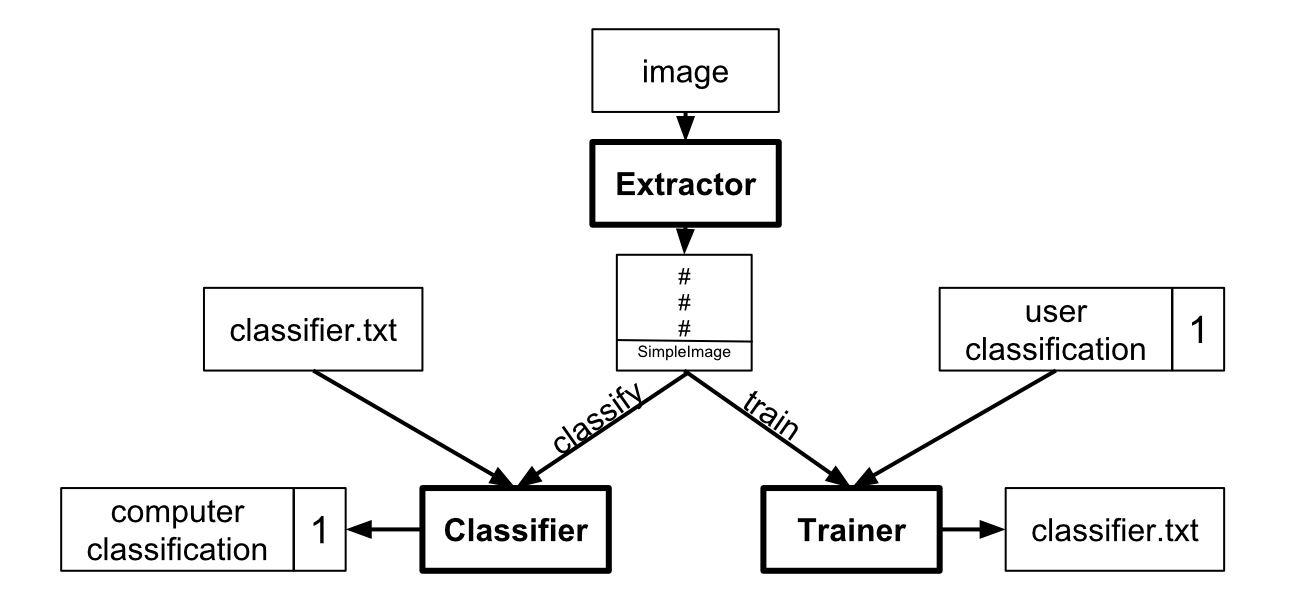
\includegraphics[width=\textwidth]{ergocr2}
    \caption{Erg OCR architechture.}
    \label{fig:ergocr}
\end{figure}

The Erg OCR system was built as an executable Python script that allowed the user to both train the system and perform OCR on images from the command line. The system is composed of three main components, the \texttt{Extractor}, the \texttt{Trainer}, and the \texttt{Classifier}. Figure \ref{fig:ergocr} gives a high level overview of these components and how they interact. \\

\begin{figure}[h]
    \centering
    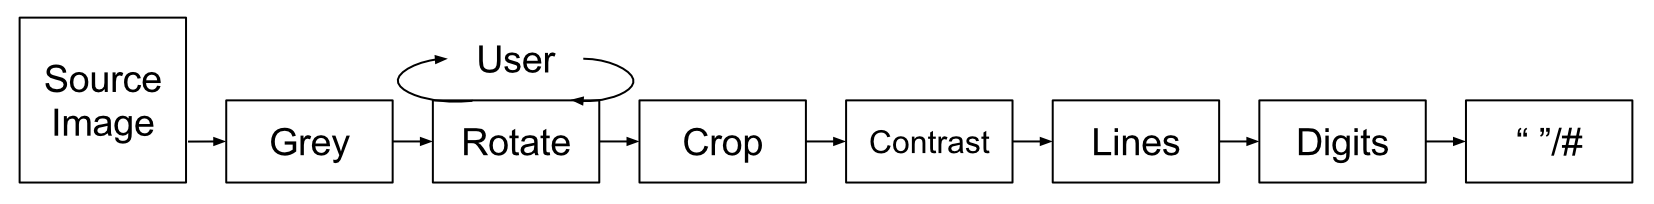
\includegraphics[width=\textwidth]{extractor2}
    \caption{The Extractor pipline.}
    \label{fig:extractor}
\end{figure}

The \texttt{Extractor} is used to both train and classify as this component finds areas of the image that it determines to be digits and allows other components to iterate through the found regions. Furthermore, the \texttt{Extractor} finds newline and tab characters in the picture and returns those as it iterates. These whitespace characters allow the system to maintain the grouping of numbers and lines. That spacing is important for interpreting the data. Figure \ref{fig:extractor} shows how the \texttt{Extractor} processes the image. First, we convert the color image to grayscale as the color data is not needed and only complicates the process. Next, we print the image to the terminal using space and \# characters and ask the user to rotate the image so the text is as horizontal as possible. After rotation, we crop the image to focus on the text-containing part of the image and resize it because we don't need the high resolution of a smartphone camera. An important step is to convert the grayscale image to purely black and white using an intensity threshold. Any pixel darker than the threshold goes to black and any pixel lighter goes to white. We determined the threshold value by experimenting with different values on different images. With a black and white image, we then split the image into lines by looking for places where there are no black pixels which indicates a line break. We repeat a similar process of looking for full white columns on each line to get individual digits. We end up with a list of 4-tuples where each tuple represents a rectangle around a found digit. We can then crop out that rectangle and create a \texttt{SimpleImage} object which is a class we created that converts black and white images to \lq \hspace{.7em} '/\# images where black is \# and white is \lq \hspace{.7em} '. This allows us to easily print the digit to the terminal. Figure \ref{fig:extraction} shows an example of these image processing steps. \\

\begin{figure}[h]
    \centering
    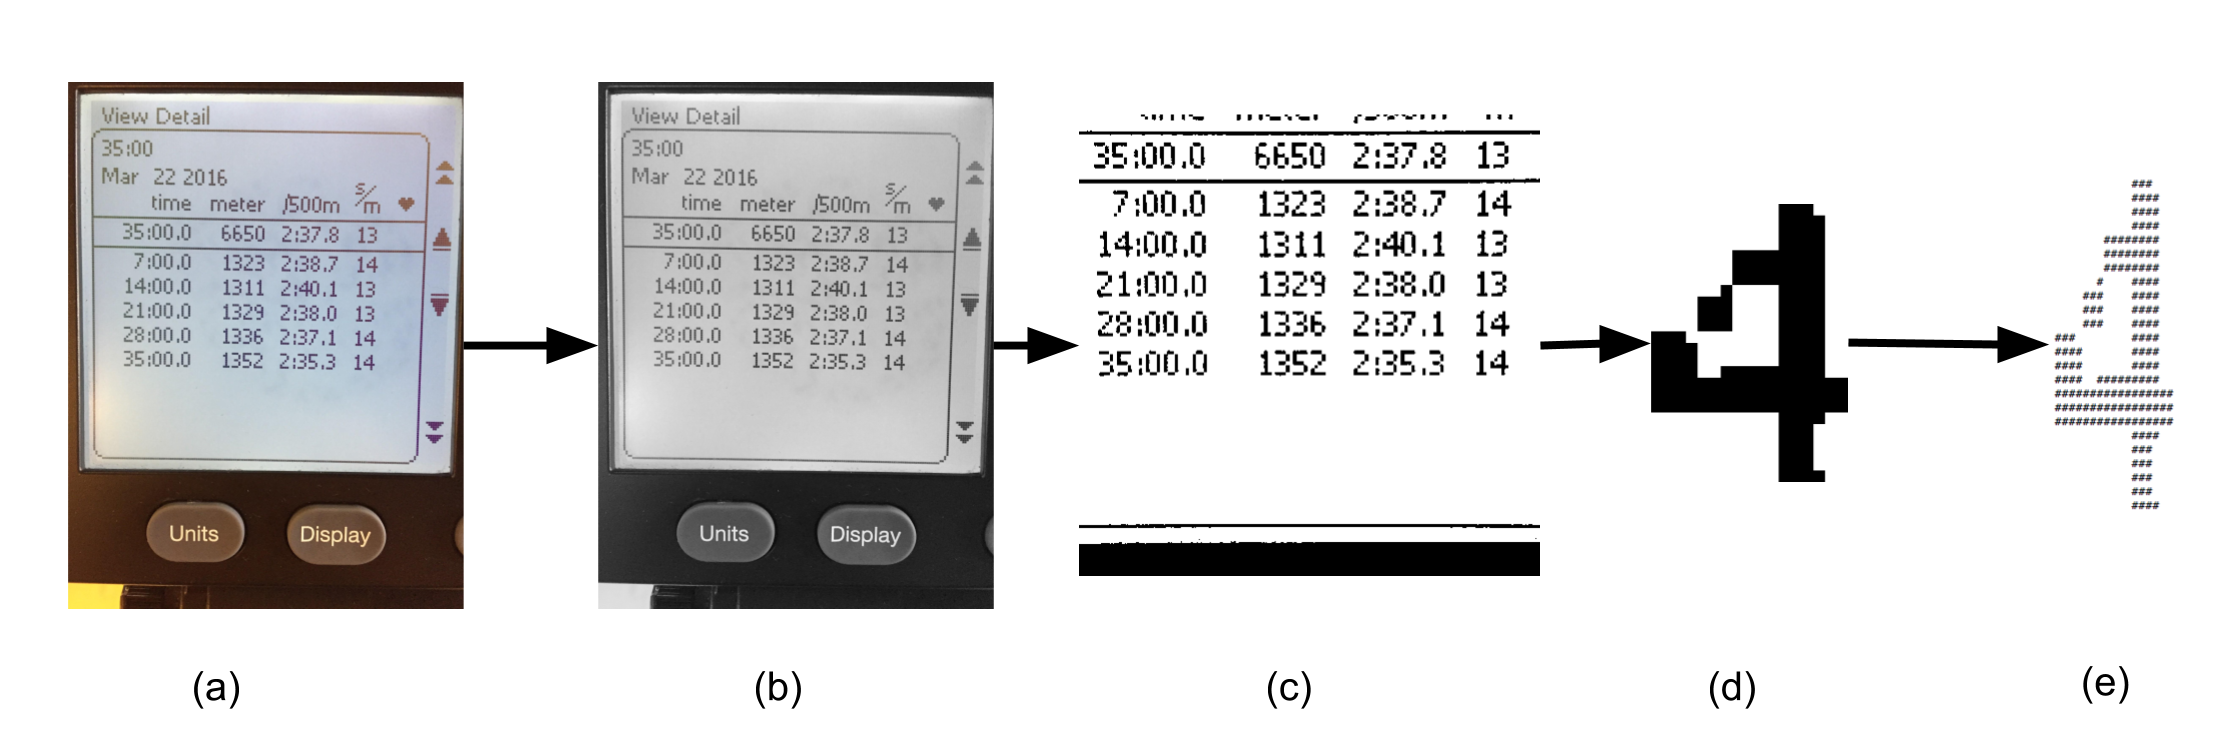
\includegraphics[width=\textwidth]{extraction}
    \caption{A example of processing an image for extraction.}
    \label{fig:extraction}
\end{figure}

To train the system, the user will need to indicate what character each pattern of pixels represents. This is the role of the \texttt{Trainer} component. The trainer first passes the image that the user wants to train through the extractor. Now the trainer iterates through each section of the image that the extractor finds to contain a digit. Since the trainer gets a \texttt{SimpleImage} from the extractor, it can easily print out the digit to the terminal as spaces and \#. The user then indicates what the printed symbol is. The trainer stores this mapping of pixels to a classification in a file. \\

To use the system to do OCR, the \texttt{Classifier} component will use a training file created by the trainer to run the kNN algorithm on the image the user wants to find characters in. Again, the process starts with the extractor finding the digits in the image. The classifier iterates through the \texttt{SimpleImage}s returned by the extractor and runs the kNN algorithm on each image and returns the classification it finds. For computing the similarity value, we count how many pixels are in the same position in both images. This is a simple measure of similarity as it does not account for differences in rotation or scale. The \texttt{Extractor} is the most important component of the system. Once the digits are extracted from the image, the process of running the kNN algorithm is not that complicated. See Appendix A for an example of the classifier performing OCR on an image. \\


The modular design of the system keeps the different parts of the system separate allowing each component to focus on performing its function correctly without worrying about how other components are working. Furthermore, if we wanted to test another machine learning algorithm such as SVM, we could easily swap out the kNN classifier for an SVN classifier. Lastly, because we rely only on a fairly simple imaging library, it would not be difficult to translate the system to other languages such as Swift if we were going to put it on a iOS device or Java if we were going to put the system on an Android device.

\section{Experiments \& Analysis}
We tested our system using leave one out cross validation. The dataset contained five images with a total of 442 characters to recognize. We created five sets of training data by leaving out the data from one image and using data from the remaining four. That left out image was then tested against the corresponding training set. That process was repeated for each of the five images. We first tested the impact of changing $k$ on the accuracy (\% correctly classified) by testing with a $k$ of 1, 3, and 5.  \\

\begin{table}[h]
  \centering
  \begin{tabular}{l|l}
      $k$ & accuracy \\ \hline
      1 & 97.5\% \\
      3 & 98.0\% \\
      5 & 98.0\%
  \end{tabular}
  \caption{Accuracy for different values of k for images in ideal conditions.}
  \label{table:acc_v_k}
\end{table}

The system performs very well in terms of correctly recognizing characters in the image as we reached an accuracy of 98\%. In fact, many of the images had an accuracy of 100\%. Changing k did not have a significant effect on the accuracy of the system. \\

The system performed so well because, although there was variation in the pictures because they were all taken by hand on independent occasions, all the pictures were taken in good lighting and were framed fairly consistently. Furthermore, during the extraction stage, the user has the ability to rotate the image, so all images were nearly perfectly rotated to have horizontal text. We looked to test how poorly rotated images (off by a couple of degrees) would impact the accuracy. \\

\begin{table}[h]
  \centering
  \begin{tabular}{l|l}
      $k$ & accuracy \\ \hline
      1 & 89.1\% \\
      3 & 88.5\% \\
      5 & 86.7\%
  \end{tabular}
  \caption{Accuracy for different values of k for incorrectly rotated images.}
  \label{table:acc_v_k_rot}
\end{table}

The results suggest that although the system maintains a fairly high level of accuracy, it is sensitive to small rotations. This result makes sense because the training set does not have any examples of rotated characters. We could run future tests to see if adding rotated data to the training set improves the performance on rotated images while maintaining high accuracy for well-rotated images. This result also highlights the importance of preprocessing. When the characters are at a consistent rotation and scale, the algorithm does very well. \\

Lastly, we wanted to examine the speed of the system. Since the kNN algorithm loops through every example in its training set, the size of that training set should determine how quickly the system can process images. To test this, we created a smaller training set. \\

\begin{table}[h]
  \centering
  \begin{tabular}{c|c|c}
      size of classifier & seconds per character & accuracy \\ \hline
      353 entries & 0.040 & 98.0\% \\
      113 entries & 0.014 & 96.7\% \\
  \end{tabular}
  \caption{Time per categorization and accuracy for different sized classifiers. Images under ideal conditions with k = 3.}
  \label{table:size_v_time}
\end{table}

This test shows a trade off between speed and accuracy. We can classify quicker by using a training set with fewer examples. However, if we reduce the number of examples too much the accuracy will suffer.

\section{Limitations \& Future Work}
Our system is limited by how well it can extract characters from the image. When we tried testing the program on images taken in poor lighting, the extractor was unable to find any characters because it was unable to create enough contrast between the characters on the screen and the background of the screen. This limitation does not apply to just lighting. As the experiments above show, slightly rotating the image has serious consequences on accuracy. Therefore, future work could go into creating a more robust image pre-processor. A pre-proccessor that is able to automatically rotate and scale images to the correct position and create contrast in different lighting conditions would help improve accuracy. Additionally, the kNN algorithm is simple and could be limited in how good it can get. First, we could enhance the similarity function to look for more complex features rather than just looking at the number of identical pixels. Future work should also look at other, more powerful, machine learning algorithms and see how they compare to our kNN implementation. \\


Since the goal of this project is to have users be able to do this logging with their smartphone rather than their desktop computer, creating a mobile app that uses this system at its core would be a next step. We are also limited by a lack of datasets. As a result, one extension could be to build a smartphone app that would initially use an early version of the OCR system, but would have users classify images for us as they would get the benefit of workout logging and we would get more data that we could use to build better versions of the OCR system. \\


Even when the OCR technology is good, there is still work that needs to be done to make the app a useful logging tool. Erg workouts can have many different formats (intervals with rest, single time, single distance), so the app should be able to determine what type of workout it is. Additionally, sometimes workouts can be so long that they span multiple screens, so logic would need to be in place to handle all these cases. Once the data is on the phone, there are many possible features that the app could implement: tracking weekly or monthly activity, tracking progress towards goals, competitions between people, performance dashboards for teams, and so on.


\section{Conclusion}
Using a simple kNN machine learning algorithm, we were able to successfully create a program that can read workout data from an erg screen. Although the system is sensitive to variations in images such as lighting, rotation, and scale, and although accuracy suffers when the image is taken in unideal situations, by improving the image pre-processing stage of the system and by expanding the training set, we would likely be able to raise the accuracy to levels above 95\% even for imperfect images. Furthermore, since we were able to achieve a rate of about 70 characters recognized per second (0.014 sec/classification), our system would be fast enough to meet our goal of being able to quickly log data. This system could be put into a iOS and Android application and would make for a functional and valuable training tool for rowers and anyone looking to quickly and seamlessly track their erg workouts.

\bibliographystyle{acm}
\bibliography{bibfile}

%\clearpage
\appendix
\section{Sample}
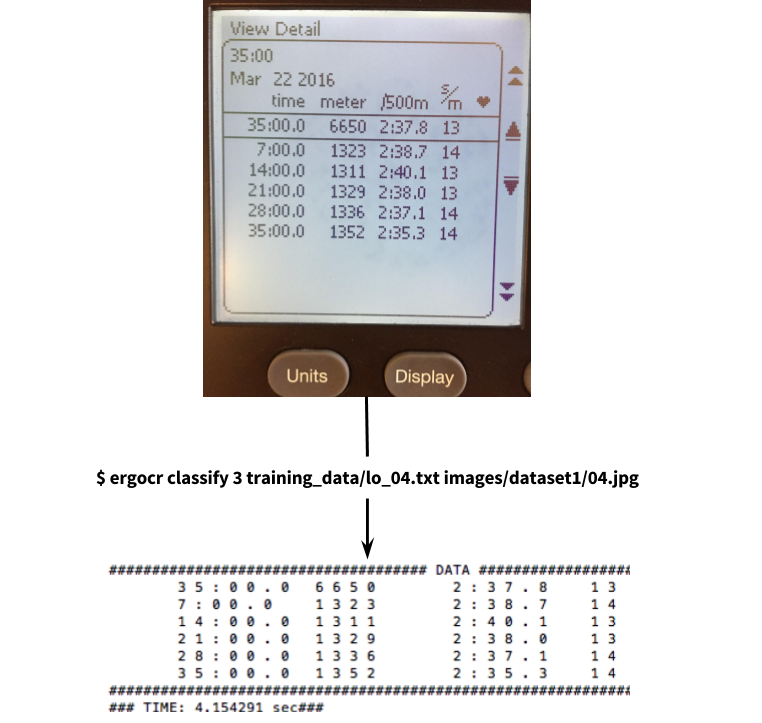
\includegraphics[width=\textwidth]{sample}



\end{document}
